\chapter{Serverless Architecture}
\label{bab:serverless}

\section*{Tujuan Pembelajaran}

\begin{enumerate}
  \item Menjelaskan pembagian antara fungsi, event, dan penjalan beserta
    kontrak yang menghubungkan ketiganya.
  \item Membedakan \textit{cold start} dari \textit{warm start}, lalu
    menentukan kapan susunan tanpa server layak dipilih.
  \item Mengukur \textit{cold start cost}, \textit{idle cost}, dan
    \textit{concurrency limit} pada penjalan fungsi dibanding layanan yang
    hidup terus.
\end{enumerate}

\section{Pendahuluan}

Seluruh bab sebelumnya memakai satu anggapan yang sama, yaitu ada proses yang
hidup terus menunggu \textit{request}. Layanan pada Bab~11 hidup sepanjang hari,
begitu pula mikroservis pada Bab~13. Anggapan itu wajar selama \textit{request}-nya
datang terus-menerus. Anggapan itu menjadi mahal ketika \textit{request}-nya jarang,
sebab proses yang menganggur tetap memegang memori dan tetap ditagih.

\textit{Serverless} membalik anggapan tersebut. Kode hanya dimuat ketika ada
kabar yang menuntutnya, dijalankan sebentar, lalu dilepas kembali. Bentuk yang
paling umum disebut Function-as-a-Service (FaaS), yaitu satuan penyebaran
berupa satu fungsi, bukan satu layanan~\cite{jonas2019berkeley}. Nama
\textit{serverless} sendiri menyesatkan, sebab servernya tetap ada. Yang hilang
adalah urusan menyediakan, menghidupkan, dan menjaga server itu, sebab
penyedialah yang mengerjakannya~\cite{cncf2018serverless}.

Bab ini memakai satu penjalan fungsi kecil yang meniru tiga fase daur hidup
AWS Lambda, yaitu \texttt{Init}, \texttt{Invoke}, dan
\texttt{Shutdown}~\cite{aws2026lambda}. Pembandingnya sebuah layanan yang hidup
terus dan menyiapkan seluruh penangannya sekali di awal. Keduanya mengerjakan
pekerjaan yang sama persis, yaitu konversi kurs, pemeriksaan pesanan, dan
penghitungan pajak, sehingga selisihnya benar-benar berasal dari cara kodenya
dimuat dan dilepas.

\section{Fungsi, Event, dan Penjalan}

Susunannya terdiri atas tiga peran. \textbf{Fungsi} adalah satu kemampuan kecil
yang menjawab satu jenis kabar. \textbf{Event} adalah kabar yang datang beserta
muatannya. \textbf{Penjalan} adalah pihak yang memuat fungsi, memanggilnya,
lalu melepasnya kembali.

Penjalan tidak mengenal satu nama fungsi pun. Yang dikenalnya hanya bentuk
kontrak beserta registri manifes. Gambar~\ref{fig:alur-serverless} menunjukkan
jalannya satu event, dan perhatikan bahwa tidak ada panah yang berangkat dari
penjalan menuju nama fungsi tertentu.

\begin{figure}[htbp]
  \centering
  \begin{tikzpicture}[
    kotak/.style={draw, rounded corners=2pt, minimum width=2.1cm,
      minimum height=0.9cm, align=center, font=\scriptsize\bfseries},
    panah/.style={-{Stealth[length=2mm]}, thick}
  ]
    \node[kotak, fill=gray!22] (event) {Event\\
      {\tiny\mdseries pajak}};
    \node[kotak, fill=praditagreen!25, right=1.0cm of event,
      minimum width=2.4cm] (penjalan) {Penjalan\\
      {\tiny\mdseries panggil()}};
    \node[kotak, fill=blue!8, above right=0.5cm and 1.1cm of penjalan]
      (registri) {Registri\\{\tiny\mdseries manifes JSON}};
    \node[kotak, fill=green!10, below right=0.5cm and 1.1cm of penjalan]
      (fungsi) {Fungsi\\{\tiny\mdseries FungsiPajak}};

    \draw[panah] (event) -- (penjalan);
    \draw[panah] (penjalan) -- node[above, font=\tiny, pos=0.55]
      {baca manifes} (registri);
    \draw[panah] (penjalan) -- node[below, font=\tiny, pos=0.55]
      {impor lalu panggil} (fungsi);
  \end{tikzpicture}
  \caption{Penjalan membaca manifes lebih dahulu, baru mengimpor modul
    fungsinya. Nama kelas fungsinya tertulis di manifes, bukan di dalam kode
    penjalan}
  \label{fig:alur-serverless}
\end{figure}

Pemisahan manifes dari modulnya bukan hiasan. Manifes berupa berkas JavaScript
Object Notation (JSON) yang memuat nama event, nama modul, nama kelas, dan
besar memori yang dipesan. Penjalan karena itu dapat mengetahui event apa saja
yang dilayani tanpa mengimpor satu baris kode fungsi pun.
Listing~\ref{lst:manifes-pajak} memperlihatkan satu manifes selengkapnya.

\begin{lstlisting}[language=bash, caption={Manifes fungsi pajak, tersedia di
  \berkas{sources/chapter14/fungsi/fungsi_pajak.json}}, label=lst:manifes-pajak]
{
  "nama": "Hitung Pajak",
  "event": "pajak",
  "keterangan": "Menghitung pajak terutang lewat tabel dua ratus ribu baris",
  "modul": "fungsi.fungsi_pajak",
  "kelas": "FungsiPajak",
  "memori_mb": 256
}
\end{lstlisting}

Kontraknya sendiri sempit, yaitu konstruktor tanpa argumen ditambah satu metode
penangan. Pembagian itu menentukan letak biaya, dan letaknya itulah yang diukur
sepanjang bab. Listing~\ref{lst:kontrak-fungsi} memuat kontraknya.

\begin{lstlisting}[style=PythonStyle, caption={Kontrak yang wajib dipenuhi
  setiap fungsi, tersedia di \berkas{sources/chapter14/kontrak.py}},
  label=lst:kontrak-fungsi]
class Fungsi(Protocol):
  """Satu kemampuan kecil yang dimuat penjalan ketika event-nya datang."""

  def __init__(self) -> None:
    """Menyiapkan seluruh bahan yang dipakai berulang oleh penangan."""

  def tangani(self, event: dict) -> dict:
    """Melayani satu event lalu mengembalikan dict berisi hasilnya."""
\end{lstlisting}

Tabel~\ref{tab:peran-serverless} merangkum tanggung jawab ketiga peran beserta
larangannya.

\begin{table}[htbp]
  \centering
  \caption{Tanggung jawab dan larangan fungsi, penjalan, serta registri}
  \label{tab:peran-serverless}
  \begin{tabularx}{\textwidth}{|l|X|X|}
    \hline
    \textbf{Peran} & \textbf{Tanggung jawab} & \textbf{Tidak boleh mengetahui} \\
    \hline
    Fungsi & Menyiapkan bahannya di konstruktor lalu melayani satu event & Siapa yang memanggilnya dan berapa lama contohnya disimpan \\
    \hline
    Penjalan & Memuat modul, memanggil penangan, lalu melepas contoh yang diam & Nama kelas mana pun, sebab namanya dibaca dari manifes \\
    \hline
    Registri & Membaca seluruh manifes lalu menjawab pertanyaan tentang event & Isi kode fungsinya, sebab manifes dibaca tanpa mengimpor \\
    \hline
  \end{tabularx}
\end{table}

Satu baris pada tabel tersebut sering terlewat, yaitu fungsi tidak tahu berapa
lama contohnya disimpan. Penyimpanan itulah yang menentukan apakah pemanggilan
berikutnya mahal atau murah, dan seksi berikutnya menjelaskannya.

\section{Tiga Fase Daur Hidup}

Satu pemanggilan menempuh paling banyak tiga fase. \textbf{Init} memuat
modulnya lalu membuat objeknya. \textbf{Invoke} memanggil penangan dengan
muatan \textit{event}-nya. \textbf{Shutdown} melepas objek yang sudah lama diam. Ketiga
nama tersebut diambil dari dokumentasi AWS Lambda, dan urutannya sama
persis~\cite{aws2026lambda}.

Listing~\ref{lst:init-shutdown} memperlihatkan kedua fase yang paling
menentukan. Fase \texttt{Init} berupa impor ditambah pembuatan objek,
sedangkan fase \texttt{Shutdown} melepas contoh yang diam melebihi batas.

\begin{lstlisting}[style=PythonStyle, caption={Fase Init dan fase Shutdown,
  tersedia di \berkas{sources/chapter14/penjalan.py}}, label=lst:init-shutdown]
def bangun_objek(self, event: str):
  """Mengimpor modul fungsinya lalu membuat objeknya, yaitu fase Init."""
  manifes = self.pendaftar.manifes_untuk(event)
  modul = importlib.import_module(manifes["modul"])
  kelas = getattr(modul, manifes["kelas"])
  return kelas()


def lepas_yang_diam(self, paksa: bool = False) -> int:
  """Melepas contoh yang diam melebihi batas, yaitu fase Shutdown."""
  sekarang = time.monotonic()
  jumlah = 0
  for event, daftar in self.kolam.items():
    bertahan = []
    for contoh in daftar:
      diam = sekarang - contoh.terakhir_dipakai
      if not contoh.sibuk and (paksa or diam >= self.batas_diam):
        jumlah += 1
      else:
        bertahan.append(contoh)
    self.kolam[event] = bertahan
    if not bertahan:
      self.lupakan_modul(event)
  return jumlah
\end{lstlisting}

Baris terakhir pada fungsi kedua itulah yang membuat turun ke nol benar-benar
terjadi. Ketika contoh terakhir sebuah fungsi dilepas, modulnya dikeluarkan
dari \textit{import cache} Python. Tanpa langkah tersebut, pemanggilan
berikutnya hanya membaca cache, sehingga \textit{cold start} terlihat jauh
lebih murah daripada yang sebenarnya.

Gambar~\ref{fig:sekuens-serverless} membandingkan satu pemanggilan dingin
dengan satu pemanggilan hangat. Jumlah langkahnya berbeda, dan selisih itulah
yang nanti terbaca sebagai angka.

\begin{figure}[htbp]
  \centering
  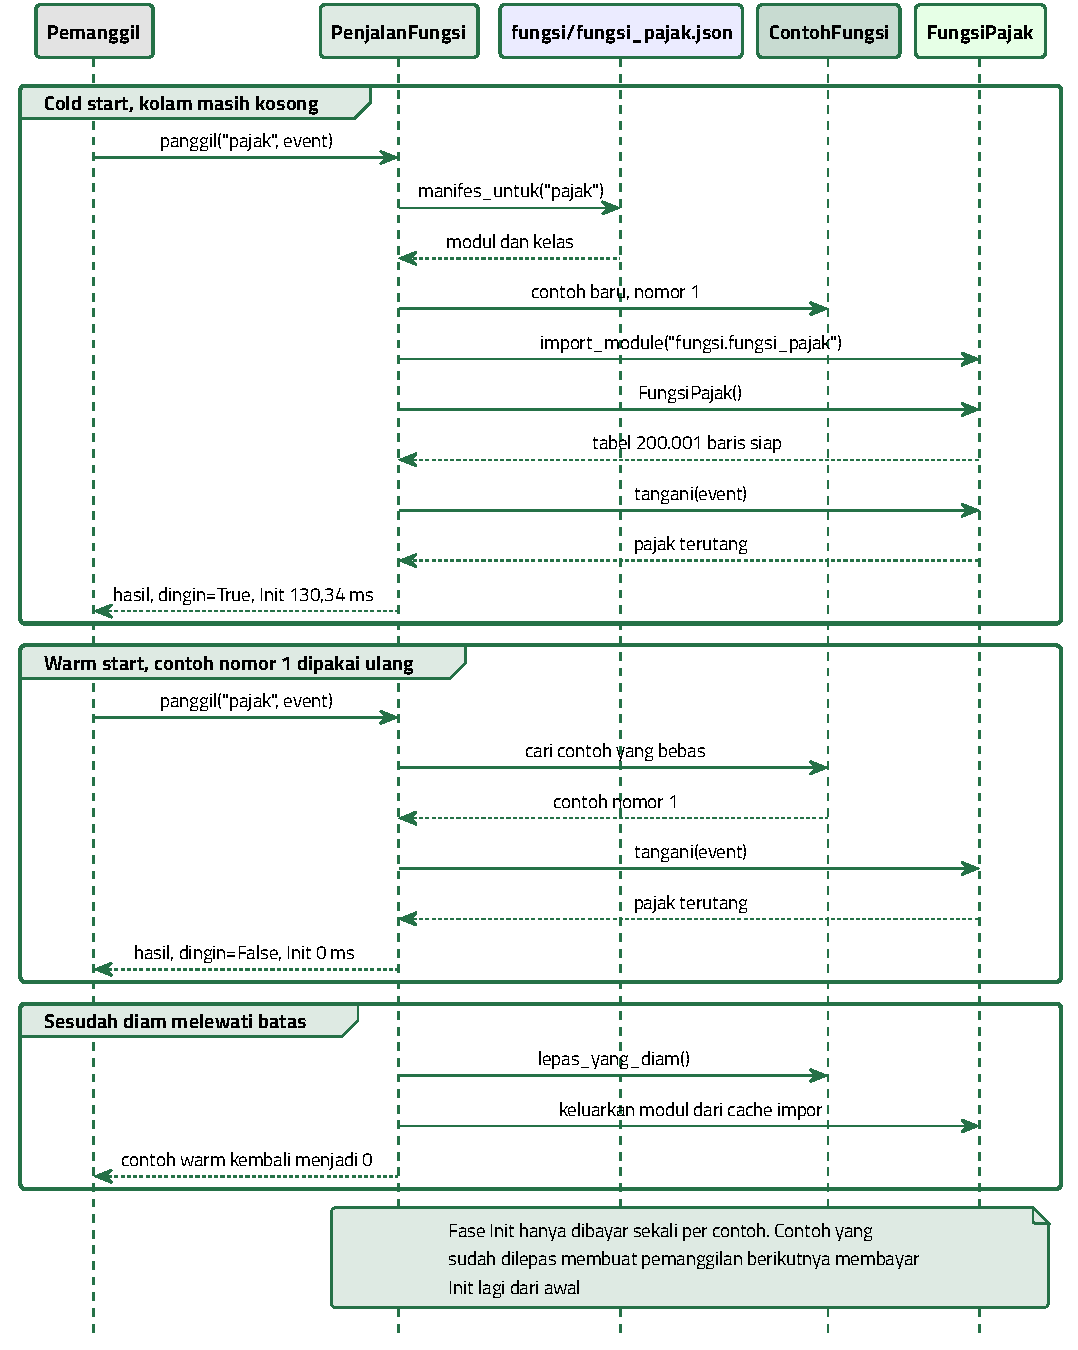
\includegraphics[width=0.92\textwidth, height=0.52\textheight,
    keepaspectratio]{sekuens-serverless.pdf}
  \caption{Pemanggilan dingin menempuh impor beserta pembuatan objek lebih
    dahulu, sedangkan pemanggilan hangat langsung masuk fase Invoke}
  \label{fig:sekuens-serverless}
\end{figure}

Menjalankan \texttt{python penjalan.py} memperlihatkan ketiga fase itu
berurutan dengan angka nyata. Pemanggilan pertama membayar
\texttt{Init} 158,713 milidetik, pemanggilan kedua membayar nol, lalu sesudah
didiamkan 2,2 detik pemanggilan ketiga membayar \texttt{Init} lagi.

\section{Mulai Dingin dan Mulai Hangat}

Pemanggilan yang menemukan contoh siap pakai disebut \textbf{\textit{warm
start}}. Pemanggilan yang harus membuat contohnya lebih dahulu disebut
\textbf{\textit{cold start}}. Perbedaan keduanya hanya satu, yaitu siapa yang
membayar fase \texttt{Init}.

Analoginya lampu koridor berpenginderaan gerak. Koridor yang kosong gelap total
dan tidak menghabiskan daya sedikit pun. Orang pertama yang lewat menunggu
sesaat sampai lampunya terang penuh. Orang berikutnya yang lewat tidak menunggu
apa pun, sebab lampunya masih menyala. Beberapa menit sesudah koridornya sepi,
lampu itu padam kembali dengan sendirinya.

Skrip \texttt{ukur\_mulai.py} menjalankan dua ratus panggilan untuk tiap
fungsi, dan setiap panggilan kelima sengaja dibuat dingin dengan melepas
contohnya lebih dahulu. Dua fungsi diukur, yaitu fungsi kurs yang persiapannya
ringan dan fungsi pajak yang menyusun tabel 200.001 baris pada fase
\texttt{Init}. Tabel~\ref{tab:mulai-dingin} memuat hasilnya.

\begin{table}[htbp]
  \centering
  \caption{\textit{Cold start} dibanding \textit{warm start}, dua ratus
    panggilan per fungsi, dalam milidetik}
  \label{tab:mulai-dingin}
  \begin{tabularx}{\textwidth}{|X|l|l|}
    \hline
    \textbf{Yang diukur} & \textbf{Fungsi kurs} & \textbf{Fungsi pajak} \\
    \hline
    Median \textit{cold start} & 0,8000 & 112,7977 \\
    \hline
    Persentil ke-95 \textit{cold start} & 1,7599 & 132,0656 \\
    \hline
    Terbesar \textit{cold start} & 4,7117 & 157,4897 \\
    \hline
    Median \textit{warm start} & 0,0040 & 0,0040 \\
    \hline
    Persentil ke-95 \textit{warm start} & 0,0146 & 0,0190 \\
    \hline
    Terbesar \textit{warm start} & 0,0722 & 0,0487 \\
    \hline
    Selisih median & 0,7961 & 112,7937 \\
    \hline
    \textit{Cold start} lebih lambat & 201,5 kali & 28.231,2 kali \\
    \hline
  \end{tabularx}
\end{table}

Tiga hal terbaca dari tabel tersebut. Pertama, median \textit{warm start}
kedua fungsi sama persis, yaitu 0,0040 milidetik, padahal persiapannya jauh
berbeda. Sebabnya persiapan yang berat sudah dibayar pada fase \texttt{Init},
sehingga penangan hanya membaca satu baris dict. Kedua, selisihnya jauh
melampaui ragam pengukurannya. \textit{Range} di dalam kelompok hangat fungsi
pajak hanya 0,0461 milidetik, yaitu 0,0004 kali selisih mediannya yang
112,7937 milidetik. Ketiga, pencacahan per panggilan menegaskannya, yaitu
seluruh 40 panggilan dingin lebih lambat daripada panggilan hangat yang paling
lambat sekalipun, pada kedua fungsi.

Angka 28.231,2 kali itu memang mencolok, dan kemencolokannya disengaja. Fungsi
pajak menyusun 200.001 baris tabel di dalam konstruktornya. Dokumentasi AWS
Lambda menyebut kode di luar penangan sebagai penyumbang terbesar latensi
sebelum fungsi berjalan, dan tabel seperti itulah contoh
khasnya~\cite{aws2026lambda}. Pertanyaannya, mengapa persiapan berat itu tidak
dipindahkan saja ke dalam penangan. Jawabannya terbaca pada baris median
\textit{warm start}, yaitu pemindahan seperti itu akan membuat setiap
pemanggilan membayar penyusunan tabel, bukan hanya pemanggilan pertama.

\section{Harga Diam dan Gigabita Detik}

Mahalnya \textit{cold start} menimbulkan pertanyaan yang wajar. Bila mulai
dingin semahal itu, mengapa proses yang hidup terus tidak dipakai saja.
Jawabannya ada pada harga yang dibayar ketika \textit{request}-nya sedang tidak
datang, dan harga itu disebut \textbf{\textit{idle cost}}.

Skrip \texttt{ukur\_sumber\_daya.py} menakar keduanya pada keadaan diam, lalu
menghitung tagihannya memakai satuan gigabita detik. Satuan itu dipakai
penyedia sungguhan, yaitu besar memori yang dipesan dikalikan lama fungsinya
berjalan~\cite{aws2026lambda}. Tabel~\ref{tab:diam-serverless} memuat hasilnya.

\begin{table}[htbp]
  \centering
  \caption{Keadaan diam kedua susunan, diukur sesudah seluruh contoh dilepas}
  \label{tab:diam-serverless}
  \begin{tabularx}{\textwidth}{|X|l|l|}
    \hline
    \textbf{Yang diukur} & \textbf{Penjalan fungsi} & \textbf{Layanan hidup} \\
    \hline
    Memori saat hangat & 21.213,0 KiB & 21.179,3 KiB \\
    \hline
    Memori saat diam & 13,1 KiB & 21.179,3 KiB \\
    \hline
    Modul fungsi yang dimuat saat diam & 0 & 3 \\
    \hline
    Prosesor saat diam & 0,059 ms & 0,041 ms \\
    \hline
    \textit{Request} pertama sesudah diam & 115,3791 ms & 0,0230 ms \\
    \hline
  \end{tabularx}
\end{table}

Baris kedua tabel itu yang paling menentukan. Penjalan menyimpan 13,1 KiB saat
diam, sedangkan layanan hidup tetap memegang 21.179,3 KiB, yaitu 1.616 kali
lebih besar. Sebabnya terbaca pada baris berikutnya, yaitu nol modul fungsi
melawan tiga modul fungsi. Kemampuan itulah yang disebut \textbf{turun ke nol},
atau \textit{scale to zero}. Harganya terbaca pada baris terakhir, yaitu
\textit{request} pertama sesudah diam membayar 115,3791 milidetik pada penjalan dan
hanya 0,0230 milidetik pada layanan hidup.

Selisih memori tersebut baru menjadi uang ketika dihitung sebagai tagihan.
Tabel~\ref{tab:gigabita-detik} memuat hitungannya pada beban 720 \textit{request} per
jam, yaitu satu \textit{request} setiap lima detik.

\begin{table}[htbp]
  \centering
  \caption{Gigabita detik per jam pada beban 720 \textit{request} per jam}
  \label{tab:gigabita-detik}
  \begin{tabularx}{\textwidth}{|l|l|l|X|}
    \hline
    \textbf{Susunan} & \textbf{Memori dipesan} & \textbf{Lama tertagih} & \textbf{Gigabita detik} \\
    \hline
    Penjalan, selalu dingin & 256 MB & 114 ms & 20,52 \\
    \hline
    Penjalan, selalu hangat & 256 MB & 1 ms & 0,18 \\
    \hline
    Layanan hidup & 512 MB & 3.600.000 ms & 1.800,00 \\
    \hline
  \end{tabularx}
\end{table}

Baris ketiga itu bukan salah ketik. Layanan yang hidup terus ditagih sepanjang
jam itu, baik ada \textit{request} maupun tidak, sehingga lama tertagihnya satu jam
penuh. Penjalan hanya ditagih selama fungsinya benar-benar berjalan, dan
lamanya dibulatkan ke atas menjadi milidetik. Perbandingannya 87,7 kali pada
keadaan selalu dingin, lalu 10.000 kali pada keadaan selalu hangat.

Keunggulan sebesar itu tidak berlaku selamanya. Titik impasnya dapat dihitung,
yaitu 63.158 \textit{request} per jam bila setiap \textit{request} membayar mulai dingin,
dan 7.200.000 \textit{request} per jam bila seluruhnya hangat. Di atas angka
tersebut, layanan yang hidup terus justru lebih murah. Pilihannya karena itu
bergantung pada kerapatan \textit{request}, bukan pada selera arsitektur.

\section{Lonjakan Serentak}

Kasus berikut memperlihatkan sisi yang belum terukur. Sebuah unit keuangan
kampus memindahkan penghitungan pajak ke fungsi tanpa server. Pada hari biasa
\textit{request}-nya 720 per jam, dan tagihannya turun dari 1.800,00 menjadi 20,52
gigabita detik. Pada penutupan semester, dua belas \textit{request} datang bersamaan
sedangkan batas contohnya hanya empat. Delapan \textit{request} menunggu giliran,
median latensinya naik menjadi 696,9689 milidetik, dan petugas loket mengira
sistemnya menggantung.

Skrip \texttt{ukur\_lonjakan.py} mengulang cerita itu sepuluh putaran, yaitu
dua belas \textit{request} serentak pada setiap putaran.
Tabel~\ref{tab:lonjakan-serverless} memuat hasilnya atas 120 \textit{request}.

\begin{table}[htbp]
  \centering
  \caption{Dua belas \textit{request} serentak, batas empat contoh, sepuluh putaran}
  \label{tab:lonjakan-serverless}
  \begin{tabularx}{\textwidth}{|X|l|l|l|}
    \hline
    \textbf{Yang diukur} & \textbf{Kolam kosong} & \textbf{Kolam hangat} & \textbf{Layanan hidup} \\
    \hline
    Contoh fungsi dibuat & 40 & 0 & 0 \\
    \hline
    \textit{Request} menunggu & 80 & 0 & 0 \\
    \hline
    Median latensi & 696,9689 ms & 0,0127 ms & 0,0037 ms \\
    \hline
    Persentil ke-95 latensi & 804,8510 ms & 0,0236 ms & 0,0070 ms \\
    \hline
    Latensi terbesar & 866,5934 ms & 0,0297 ms & 0,0123 ms \\
    \hline
  \end{tabularx}
\end{table}

Dua angka pada kolom pertama menjelaskan seluruh kolomnya. Empat contoh dibuat
pada setiap putaran, sebab batas kesertaan, atau \textit{concurrency limit},
memang empat. Delapan \textit{request} sisanya menunggu sampai ada contoh yang
selesai. Median latensinya karena itu 54.879 kali median kolam hangat, padahal
pekerjaan domainnya sama persis.

Kolom kedua memperlihatkan bahwa lonjakan itu sendiri bukan penyebabnya. Dua
belas \textit{request} serentak pada kolam yang sudah hangat tidak membuat satu
contoh baru pun, dan tidak satu \textit{request} pun menunggu. Yang mahal adalah
lonjakan yang datang ketika kolamnya kosong, yaitu persis keadaan sesudah
sistemnya turun ke nol.

\section{Biaya Menambah Fungsi}

Ukuran terakhir bab ini adalah biaya perubahan. Bagian penjualan meminta satu
kemampuan baru, yaitu penghitungan diskon. Skrip \texttt{ukur\_perubahan.py}
menambahkan fungsi tersebut pada kedua susunan, lalu menghitung berkas dan
baris yang tersentuh. Tabel~\ref{tab:ubah-serverless} memuat hasilnya.

\begin{table}[htbp]
  \centering
  \caption{Biaya menambah satu fungsi baru pada kedua susunan}
  \label{tab:ubah-serverless}
  \begin{tabularx}{\textwidth}{|X|l|l|}
    \hline
    \textbf{Yang diukur} & \textbf{Penjalan fungsi} & \textbf{Layanan hidup} \\
    \hline
    Berkas baru yang ditambahkan & 2 & 2 \\
    \hline
    Baris kodenya & 363 & 83 \\
    \hline
    Baris yang menyebut nama fungsi & 0 & 6 \\
    \hline
    Baris yang disunting demi fungsi baru & 0 & 2 \\
    \hline
  \end{tabularx}
\end{table}

Baris ketiga itulah pokoknya. Penjalan sepanjang 363 baris tidak menyebut satu
nama fungsi pun, sehingga fungsi baru cukup berupa dua berkas, yaitu satu modul
dan satu manifes. Layanan hidup yang hanya 83 baris justru menyebut nama
fungsinya pada enam baris, yaitu dua baris untuk tiap fungsi, sehingga fungsi
keempat menuntut dua baris suntingan di dalamnya.

Gambar~\ref{fig:kelas-serverless} menunjukkan hubungan kelasnya. Perhatikan
bahwa tidak ada panah yang berangkat dari penjalan menuju ketiga fungsi,
sedangkan panah dari registri menuju manifes justru ada.

\begin{figure}[htbp]
  \centering
  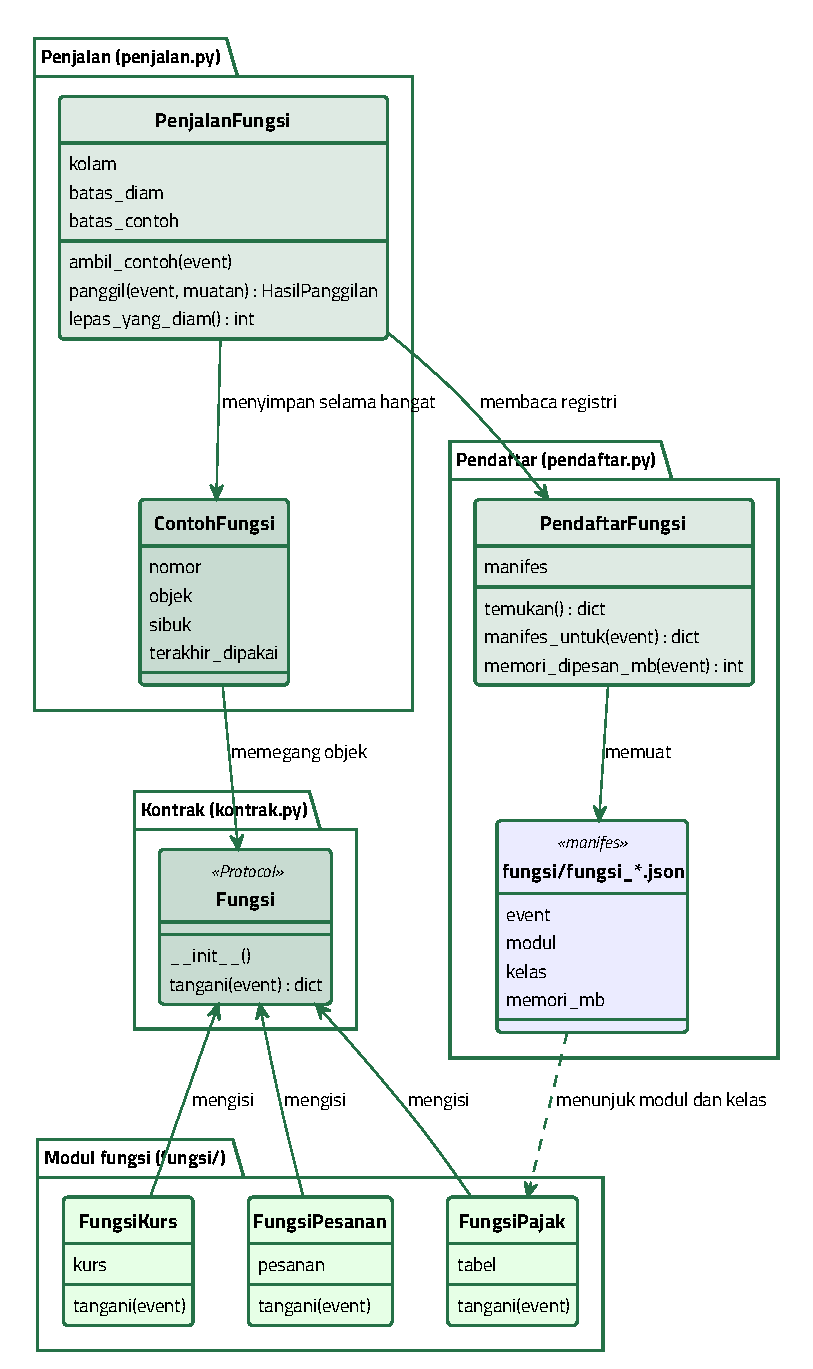
\includegraphics[width=\textwidth, height=0.60\textheight,
    keepaspectratio]{kelas-serverless.pdf}
  \caption{Penjalan hanya mengenal kontrak beserta registri manifes, sedangkan
    nama kelas setiap fungsi tertulis di dalam manifesnya}
  \label{fig:kelas-serverless}
\end{figure}

Kemurahan itu bukan hadiah gratis. Nama kelas yang berpindah dari kode ke
manifes membuat kesalahan ketik tidak lagi tertangkap pada saat impor,
melainkan pada saat event pertamanya datang. Pertukarannya sama seperti pada
Bab~5, yaitu kelenturan ditebus dengan pemeriksaan yang bergeser ke waktu
jalan.

\section{\textit{Summary}}

\textit{Serverless} memindahkan urusan menghidupkan dan menjaga proses kepada
penyedia. Satuan penyebarannya satu fungsi, dan fungsi itu hanya dimuat ketika
event-nya datang. Penjalan pada bab ini meniru tiga fase AWS Lambda, yaitu
\texttt{Init} yang memuat modul, \texttt{Invoke} yang memanggil penangan, dan
\texttt{Shutdown} yang melepas contoh yang diam.

Pemuatan yang ditunda itu dibayar pada pemanggilan pertama. Median
\textit{cold start} fungsi pajak tercatat 112,7977 milidetik melawan 0,0040
milidetik pada \textit{warm start}, yaitu 28.231,2 kali. Seluruh 40 panggilan
dingin lebih lambat daripada panggilan hangat yang paling lambat sekalipun,
sehingga selisihnya tidak dapat disebut kebetulan. Besarnya ditentukan isi
konstruktor, sebab fungsi kurs yang persiapannya ringan hanya membayar 0,8000
milidetik.

Yang dibeli dengan pembayaran itu terbaca pada keadaan diam. Penjalan menyimpan
13,1 KiB dan nol modul fungsi, sedangkan layanan hidup tetap memegang 21.179,3
KiB beserta ketiga modulnya. Pada beban 720 \textit{request} per jam, tagihannya
20,52 gigabita detik melawan 1.800,00 gigabita detik, dan titik impasnya
63.158 \textit{request} per jam.

Harga lain muncul ketika \textit{request}-nya datang bersamaan. Dua belas \textit{request}
serentak pada kolam yang kosong membuat delapan \textit{request} menunggu, dan median
latensinya 696,9689 milidetik. Lonjakan yang sama pada kolam yang sudah hangat
tidak membuat satu contoh baru pun. Yang mahal karena itu bukan lonjakannya,
melainkan lonjakan yang menimpa sistem yang baru saja turun ke nol.

Pesan utama bab ini karena itu bukan bahwa tanpa server selalu lebih murah,
melainkan bahwa tanpa server memindahkan biaya dari waktu diam ke waktu mulai.
Pemindahan itu menguntungkan selama \textit{request}-nya jarang, dan merugikan ketika
\textit{request}-nya rapat atau datang serentak. Ketiga angka pada bab ini, yaitu
\textit{cold start}, gigabita detik, dan \textit{request} yang menunggu, adalah dasar
untuk menimbang keduanya.

\section{Latihan}

Ketiga latihan berikut memakai satu basis kode yang sama di
\berkas{sources/chapter14/}, tetapi menyasar tiga masalah yang berbeda.
Latihan~1 mengukur \textit{cold start cost}. Latihan~2 mengukur
\textit{idle cost} beserta titik impasnya. Latihan~3 mengukur
\textit{concurrency limit} ketika \textit{request}-nya datang serentak. Hasil setiap
mahasiswa dapat berbeda, dan yang dilaporkan adalah pola perbandingannya, bukan
angka mutlaknya.

Venv yang sama dipakai kembali, dan pengaktifannya seperti pada
Listing~\ref{lst:venv-ch14}. Bab ini hanya memakai pustaka standar Python,
sehingga tidak ada pemasangan tambahan.

\begin{lstlisting}[language=bash, caption={Menyiapkan bahan sebelum ketiga
  latihan, seluruh skrip tersedia di \berkas{sources/chapter14/}},
  label=lst:venv-ch14]
bash sources/siapkan_venv.sh
source .venv/bin/activate
cd sources/chapter14
python penjalan.py
# Keluarannya: Panggilan 1 dingin=True Init 158.713 ms  tangani 0.019 ms
#              Panggilan 2 dingin=False Init 0.000 ms  tangani 0.004 ms
#              Contoh dibuat seluruhnya : 2
#              Contoh dilepas seluruhnya: 1
\end{lstlisting}

\subsection*{Latihan 1: \textit{Cold Start Cost}}

Latihan ini menguji klaim yang sering diucapkan tanpa angka, yaitu mulai dingin
hanya persoalan kecil. Klaim itu menyebut angka, sehingga dapat dibuktikan
salah. Langkah kerjanya sebagai berikut.

\begin{enumerate}
  \item Jalankan perintah pada Listing~\ref{lst:jalankan-mulai}, lalu catat
    kedelapan angka latensi kedua fungsi.
  \item Catat baris \texttt{Range dibagi selisih} beserta baris
    \texttt{Dingin melebihi hangat terbesar} pada kedua fungsi.
  \item Buka \berkas{sources/chapter14/fungsi/fungsi_pajak.py}, lalu tunjukkan
    baris yang membuat fase \texttt{Init} menjadi berat.
  \item Ubah \texttt{LANGKAH\_TABEL} dari 1.000 menjadi 100, jalankan ulang,
    lalu catat perubahan median \textit{cold start} fungsi pajak. Kembalikan
    nilainya sesudah dicatat.
\end{enumerate}

\begin{lstlisting}[language=bash, caption={Mengukur \textit{cold start cost},
  skrip tersedia di \berkas{sources/chapter14/ukur_mulai.py}},
  label=lst:jalankan-mulai]
python ukur_mulai.py
# Keluarannya: Median mulai dingin          : 112.7977 ms
#              Median mulai hangat          : 0.0040 ms
#              Mulai dingin lebih lambat    : 28231.2 kali
#              Range dibagi selisih         : 0.0004 kali
#              Dingin melebihi hangat terbesar : 40 dari 40
\end{lstlisting}

Tabel~\ref{tab:lat1serverless-contoh} berisi hasil satu kali pengukuran nyata.

\begin{table}[htbp]
  \centering
  \caption{Contoh hasil Latihan 1 yang sudah terisi, dua ratus panggilan per
    fungsi}
  \label{tab:lat1serverless-contoh}
  \begin{tabularx}{\textwidth}{|X|l|l|}
    \hline
    \textbf{Yang dilaporkan} & \textbf{Fungsi kurs} & \textbf{Fungsi pajak} \\
    \hline
    Median \textit{cold start} & 0,8000 ms & 112,7977 ms \\
    \hline
    Median \textit{warm start} & 0,0040 ms & 0,0040 ms \\
    \hline
    Terbesar \textit{cold start} & 4,7117 ms & 157,4897 ms \\
    \hline
    \textit{Cold start} lebih lambat & 201,5 kali & 28.231,2 kali \\
    \hline
    \textit{Range} dibagi selisih & 0,0885 kali & 0,0004 kali \\
    \hline
    Dingin melebihi hangat terbesar & 40 dari 40 & 40 dari 40 \\
    \hline
  \end{tabularx}
\end{table}

Isikan hasil pengukuran pada Tabel~\ref{tab:lat1serverless-hasil}.

\begin{table}[htbp]
  \centering
  \caption{Lembar isian Latihan 1}
  \label{tab:lat1serverless-hasil}
  \begin{tabularx}{\textwidth}{|X|l|l|}
    \hline
    \textbf{Yang dilaporkan} & \textbf{Fungsi kurs} & \textbf{Fungsi pajak} \\
    \hline
    Median \textit{cold start} & \dots & \dots \\
    \hline
    Median \textit{warm start} & \dots & \dots \\
    \hline
    \textit{Range} dibagi selisih & \dots & \dots \\
    \hline
    Median \textit{cold start} pada langkah 100 & \dots & \dots \\
    \hline
  \end{tabularx}
\end{table}

Jawab tiga pertanyaan berikut dengan menunjuk angka pada tabel. Pertama,
jelaskan mengapa median \textit{warm start} kedua fungsi sama persis padahal
persiapannya jauh berbeda. Kedua, bandingkan \textit{range} kelompok dingin
dengan selisih mediannya, lalu jelaskan mengapa selisih itu layak disebut ada.
Ketiga, sebutkan apa yang terjadi pada median \textit{cold start} ketika
tabelnya diperbesar sepuluh kali, lalu jelaskan sebabnya.

\subsection*{Latihan 2: \textit{Idle Cost}}

Latihan ini mengukur harga yang dibayar ketika \textit{request}-nya sedang tidak
datang. Kegagalan membaca harga itu adalah sebab paling sering mengapa
pemindahan ke tanpa server tidak menghemat apa pun. Langkah kerjanya sebagai
berikut.

\begin{enumerate}
  \item Jalankan perintah pada Listing~\ref{lst:jalankan-diam}, lalu catat
    kelima baris keadaan diam kedua susunan.
  \item Catat ketiga baris gigabita detik beserta kedua baris titik impasnya.
  \item Buka \berkas{sources/chapter14/fungsi/fungsi_pajak.json}, lalu ubah
    \texttt{memori\_mb} dari 256 menjadi 512. Jalankan ulang, lalu catat
    perubahan gigabita detik dan titik impasnya. Kembalikan nilainya sesudah
    dicatat.
  \item Hitung sendiri berapa \textit{request} per jam yang membuat kedua susunan
    seharga sama, lalu bandingkan dengan baris titik impas yang dicetak skrip.
\end{enumerate}

\begin{lstlisting}[language=bash, caption={Mengukur \textit{idle cost}, skrip
  tersedia di \berkas{sources/chapter14/ukur_sumber_daya.py}},
  label=lst:jalankan-diam]
python ukur_sumber_daya.py
# Keluarannya: Memori penjalan saat nol      : 13.1 KiB
#              Memori layanan saat menganggur: 21179.3 KiB
#              Gigabita detik penjalan dingin: 20.52
#              Gigabita detik layanan hidup  : 1800.00
#              Titik impas bila dingin       : 63,158 request per jam
\end{lstlisting}

Tabel~\ref{tab:lat2serverless-contoh} berisi hasil satu kali pengukuran nyata.

\begin{table}[htbp]
  \centering
  \caption{Contoh hasil Latihan 2 yang sudah terisi, beban 720 \textit{request} per
    jam}
  \label{tab:lat2serverless-contoh}
  \begin{tabularx}{\textwidth}{|X|l|l|}
    \hline
    \textbf{Yang dilaporkan} & \textbf{Penjalan fungsi} & \textbf{Layanan hidup} \\
    \hline
    Memori saat diam & 13,1 KiB & 21.179,3 KiB \\
    \hline
    Modul fungsi saat diam & 0 & 3 \\
    \hline
    \textit{Request} pertama sesudah diam & 115,3791 ms & 0,0230 ms \\
    \hline
    Gigabita detik per jam & 20,52 & 1.800,00 \\
    \hline
    Titik impas & 63.158 per jam & tidak berlaku \\
    \hline
  \end{tabularx}
\end{table}

Isikan hasil pengukuran pada Tabel~\ref{tab:lat2serverless-hasil}.

\begin{table}[htbp]
  \centering
  \caption{Lembar isian Latihan 2}
  \label{tab:lat2serverless-hasil}
  \begin{tabularx}{\textwidth}{|X|l|l|}
    \hline
    \textbf{Yang dilaporkan} & \textbf{Memori 256 MB} & \textbf{Memori 512 MB} \\
    \hline
    Gigabita detik penjalan dingin & \dots & \dots \\
    \hline
    Gigabita detik penjalan hangat & \dots & \dots \\
    \hline
    Titik impas bila dingin & \dots & \dots \\
    \hline
    Memori penjalan saat nol & \dots & \dots \\
    \hline
  \end{tabularx}
\end{table}

Jawab tiga pertanyaan berikut dengan menunjuk angka pada tabel. Pertama,
jelaskan mengapa lama tertagih layanan hidup satu jam penuh, sedangkan lama
tertagih penjalan hanya beberapa milidetik. Kedua, sebutkan apa yang berubah
pada titik impas ketika memori yang dipesan digandakan, lalu jelaskan arah
perubahannya. Ketiga, tentukan pada kerapatan \textit{request} seperti apa layanan
yang hidup terus justru lebih murah, lalu sebutkan angka yang menjadi dasarnya.

\subsection*{Latihan 3: \textit{Concurrency Limit}}

Latihan ini membuktikan bahwa biaya terbesar tanpa server tidak muncul pada
\textit{request} yang berurutan, melainkan pada \textit{request} yang datang bersamaan
ketika kolamnya kosong. Langkah kerjanya sebagai berikut.

\begin{enumerate}
  \item Jalankan perintah pada Listing~\ref{lst:jalankan-lonjakan}, lalu catat
    kelima baris hasil ketiga keadaannya.
  \item Bandingkan baris \texttt{Request menunggu} pada ketiga keadaan, lalu
    jelaskan mengapa kolam hangat tidak membuat satu contoh baru pun.
  \item Buka \berkas{sources/chapter14/penjalan.py}, lalu naikkan
    \texttt{BATAS\_CONTOH} dari 4 menjadi 12. Jalankan ulang, lalu catat
    perubahan \textit{request} yang menunggu beserta median latensinya.
  \item Kembalikan \texttt{BATAS\_CONTOH} menjadi 4, lalu naikkan
    \texttt{JUMLAH\_SERENTAK} pada \berkas{sources/chapter14/ukur_lonjakan.py}
    dari 12 menjadi 24. Catat perubahan median latensinya.
\end{enumerate}

\begin{lstlisting}[language=bash, caption={Mengukur \textit{concurrency limit},
  skrip tersedia di \berkas{sources/chapter14/ukur_lonjakan.py}},
  label=lst:jalankan-lonjakan]
python ukur_lonjakan.py
# Keluarannya: Keadaan : penjalan, kolam kosong
#              Contoh fungsi dibuat          : 40
#              Request menunggu           : 80
#              Median latensi                : 696.9689 ms
#              Median latensi, kolam hangat  : 0.0127 ms
\end{lstlisting}

Tabel~\ref{tab:lat3serverless-contoh} berisi hasil satu kali percobaan nyata.

\begin{table}[htbp]
  \centering
  \caption{Contoh hasil Latihan 3 yang sudah terisi, 120 \textit{request}}
  \label{tab:lat3serverless-contoh}
  \begin{tabularx}{\textwidth}{|X|l|l|l|}
    \hline
    \textbf{Yang dilaporkan} & \textbf{Kolam kosong} & \textbf{Kolam hangat} & \textbf{Layanan hidup} \\
    \hline
    Contoh fungsi dibuat & 40 & 0 & 0 \\
    \hline
    \textit{Request} menunggu & 80 & 0 & 0 \\
    \hline
    Median latensi & 696,9689 ms & 0,0127 ms & 0,0037 ms \\
    \hline
    Persentil ke-95 latensi & 804,8510 ms & 0,0236 ms & 0,0070 ms \\
    \hline
    Latensi terbesar & 866,5934 ms & 0,0297 ms & 0,0123 ms \\
    \hline
  \end{tabularx}
\end{table}

Isikan hasil percobaan pada Tabel~\ref{tab:lat3serverless-hasil}.

\begin{table}[htbp]
  \centering
  \caption{Lembar isian Latihan 3}
  \label{tab:lat3serverless-hasil}
  \begin{tabularx}{\textwidth}{|X|l|l|}
    \hline
    \textbf{Yang dilaporkan} & \textbf{Batas 4 contoh} & \textbf{Batas 12 contoh} \\
    \hline
    Contoh fungsi dibuat & \dots & \dots \\
    \hline
    \textit{Request} menunggu & \dots & \dots \\
    \hline
    Median latensi & \dots & \dots \\
    \hline
    Median latensi pada 24 serentak & \dots & \dots \\
    \hline
  \end{tabularx}
\end{table}

Jawab tiga pertanyaan berikut. Pertama, jelaskan mengapa median latensi kolam
kosong ribuan kali median kolam hangat, padahal pekerjaan domainnya sama
persis. Kedua, sebutkan apa yang terjadi ketika batas contohnya dinaikkan
menjadi dua belas, lalu jelaskan mengapa menaikkan batas itu tidak gratis bagi
penyedia maupun bagi tagihan. Ketiga, dengan menggabungkan hasil ketiga
latihan, tentukan kapan susunan tanpa server layak dipilih untuk layanan kampus
yang \textit{request}-nya menumpuk pada jam tertentu, lalu sebutkan tiga angka yang
menjadi dasar keputusannya.
